\documentclass{article}[11pt]

\usepackage{graphicx}

\author{Chris Ostrouchov}
\title{Asignment 4}
\date{}

\begin{document}

\maketitle

\section{Introduction}

Homework 4 was an assignment meant for us to become more familiar with PETSc and GPU computing. PETSc is a library that has many functions that allow for the solving of linear systems iterative. As opposed to the dense linear solvers found in LAPACK. For the first part of the assignment we were required to solve a linear system using three iterative methods namely: gmres, conjugate gradient, and tfqmr. We were to then compare the run time, error of Ax - b , and number of iterations for convergence. Next we were to re-implement the cholesky QR factorization in the previous assignment using a hybrid GPU approach. This approach shows significant speedup since a GPU can be thought of a high throughput device for our costly matrix multiplications forming G. Results of comparison between the naive geqrf, cpu cholesky qr, and hybrid cholesky qr are comparred.

I have listed important specifications of the Intel i5 CPU used and Nvidia GPU used.

\begin{table}[!ht]
  \centering
  \caption{Relevant processor specifications for the Intel i5 3570k processor}
  \label{tab:i5_3570k}

  \vspace{3mm}
  \begin{tabular}{ l | l } 
    Processor & i5 3570k \\
    Clock Rate & 3.4 GHz \\
    Cores & 4 \\
    Hyper Threading & no \\
    L1 Data Cache & 4 x 32 KB \\
    L1 Latency & 4 cycles \\
    L2 Data Cache & 4 x 256 KB \\
    L2 Latency & 11 cycles \\
    L3 Data Cache & 6 MB shared \\
    L3 Latency & 28 cycles \\
    Flops / Cycle & 8 double precision
  \end{tabular}
\end{table}

\begin{table}[!ht]
  \centering
  \caption{Relevant gpu specifications for the GeForce 660}
  \label{tab:gtx_660}

  \vspace{3mm}
  \begin{tabular}{ l | l }
    GPU & GeForce GTX 660 \\
    Compute Capability & 4.0 \\
    CUDA Cores & 960 \\
    Peak Memory Rage & 6008 MHz \\
    Total Memory & 2048 MB \\
    Peak Clock Rate & 1293 MHz \\
    Peak Flops & 1881.6 GFLOPS \\
  \end{tabular}
\end{table}

\section{Results/Discussion}

Figure \ref{fig:petsc_methods} clearly shows that the conjugate gradient method is the optimal method for solving a dense random set of linear equations. However, the difference between the methods becomes less apparent as the number of itterations increase. We also see that conjugate gradient has significantly better error resolutions.

Now we are to compare the differing cholesky QR factorizations. It is expected that our cholesky qr factorization will always be more efficient than the general qr factorization provided by LAPACK since we are working with extremely overdetermined systems of equations (m >> n). This assumption greatly reduces a problem of size m >> n to a much smaller n by n problem for most of the what would be normally costly opperations such as the svd, qr, and inverse calculation. Refering to Figure \ref{fig:qr_flops}, we see that using GPUs for the hybrid approach of computing G allows for a speedup of over 10x. Proof that both the GPU and CPU implementations of the cholesky QR factorization being equal can be seen since the error for both implementations are equal. The mflops performace of the GPU code was determined using the comparable cpu opperations and dividing by the time. 

\begin{figure}
  \centering
  \caption{Comparision of PETSc methods for solving a linear system of equations. (a) Plotted with respect to time [sec] (b) Plotted with respect to error Ax - b. (c) Plotted with respect to number of Iterations for given method}
  \label{fig:petsc_methods}

  \includegraphics[width=0.50\textwidth]{../img/Time.png}
  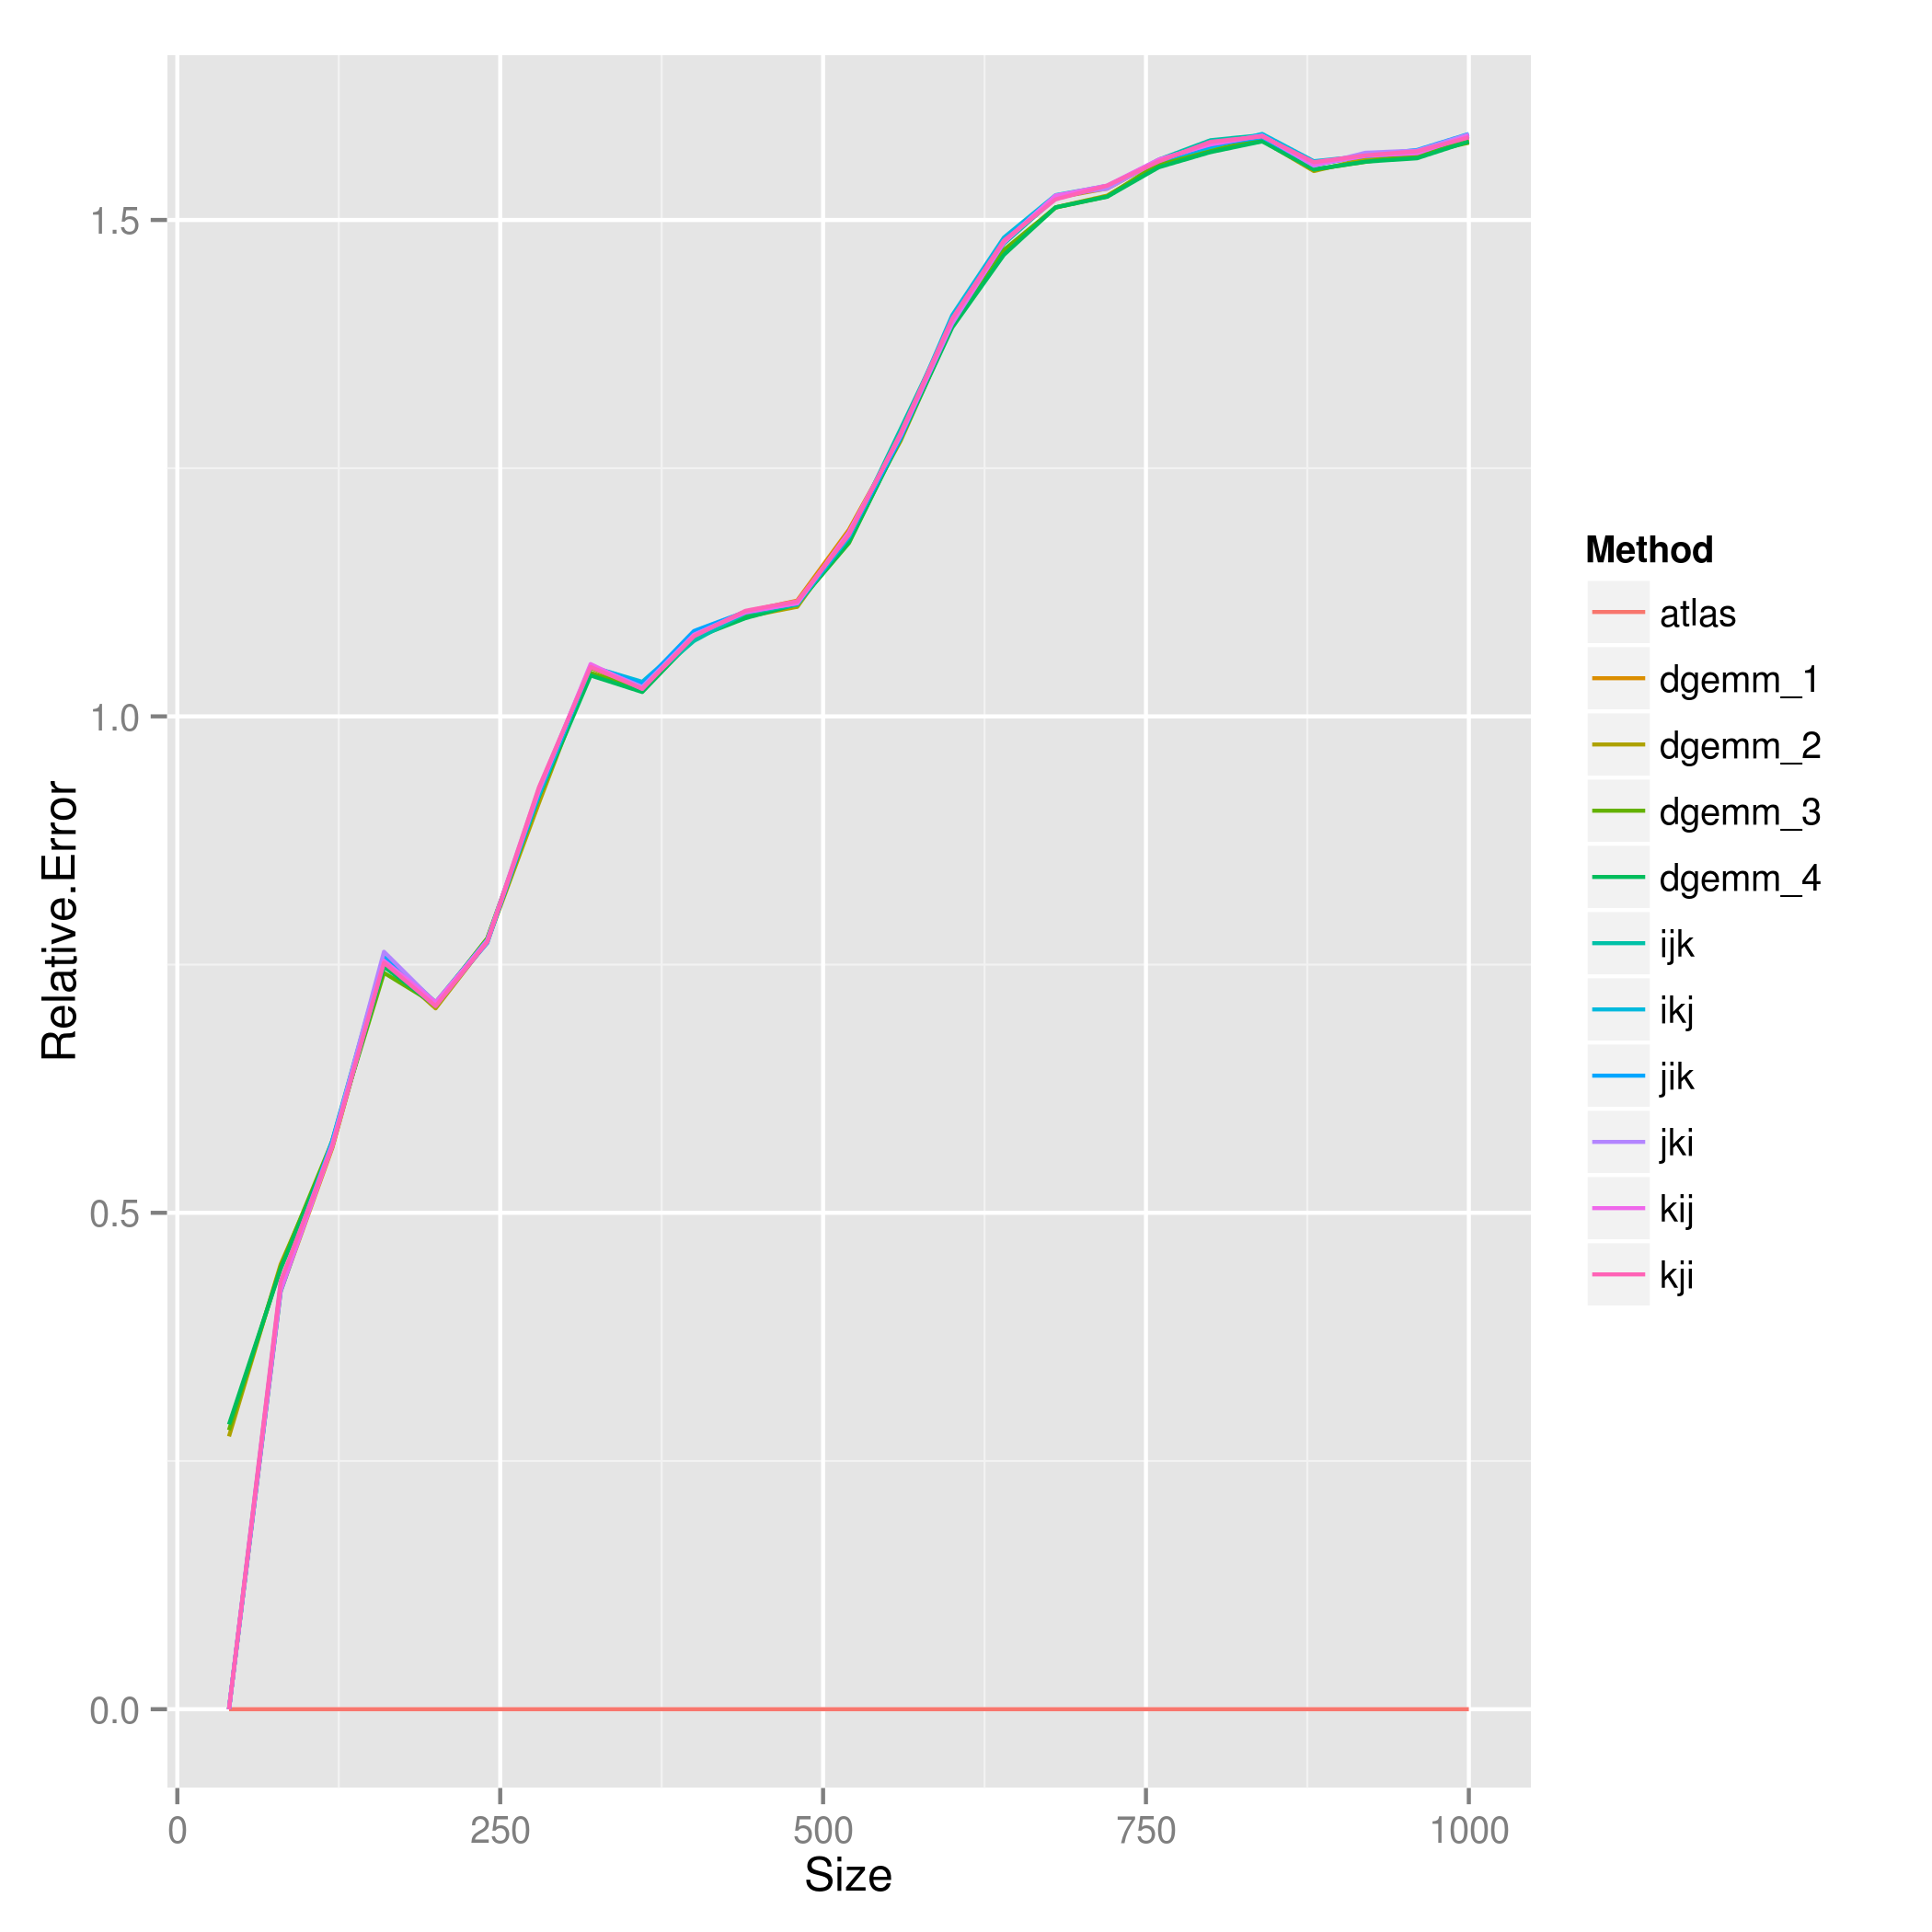
\includegraphics[width=0.50\textwidth]{../img/Error.png}
  \includegraphics[width=0.50\textwidth]{../img/Itterations.png}
\end{figure}

\begin{figure}
  \centering
  \caption{Comparision of flops performace of differing QR factorizations}
  \label{fig:qr_flops}

  \includegraphics[width=1.00\textwidth]{../img/gpu_flops.png}
\end{figure}

\begin{figure}
  \centering
  \caption{Comparision of error for differing QR factorizations}
  \label{fig:qr_error}

  \includegraphics[width=1.00\textwidth]{../img/gpu_error.png}
\end{figure}


\end{document}
